%!TEX program = xelatex
%!BIB program = bibtex


\documentclass[cn,black,10pt,normal]{elegantnote}
\usepackage{float}
\usepackage{hyperref}


%\newcommand{\upcite}[1]{\textsuperscript{\textsuperscript{\cite{#1}}}}

\title{数码摄影作业(09)摄影艺术家\\\small{Wayne F. Miller}}
\author{姓名:姜文渊\\学号:1951510}
%\institute{School of Life Science, Tongji University}
%\version{1.00}
\date{2021年5月9日}

\begin{document}

\maketitle


\section{简介}

韦恩$\cdot$米勒(Wayne Forest Miller)是美国摄影艺术家,他的照片集《北黑人的生活方式》(\textit{The Way of Life of the Northern Negro})是他广为流传的作品。\cite{wiki:Wayne_F._Miller} 

韦恩$\cdot$米勒于1918年9月19日出生于芝加哥,
他大学毕业后成为一名兼职摄影师,并于1941年至1942年间在洛杉矶艺术中心进修摄影专业。
\textbf{二次世界大战期间他在美国海军服役,拍摄记录了许多珍贵的太平洋战区战事照片。}
1958年,米勒加入马格南图片社(Magnum Photos),并在1962年至1966年期间担任马格南图片社总裁一职。
退休后,他加入到环保事业中,致力于保护加州的红木林。红木林几乎成为米勒退休后拍摄的唯一题材,直至他于2013年逝世。

下面笔者将展示几幅他在\textbf{二战期间拍摄的作品}。
\begin{figure}[H]
    \centering
    
\includegraphics[width=0.5\textwidth]{F1}
    \caption{From “Pacific Theater,” WWII, 1942-45 \\ 路易斯·蒙巴顿勋爵上将在萨拉托加号上向人员致辞}
    \label{F-02}
\end{figure}

\begin{figure}[H]
    \centering
    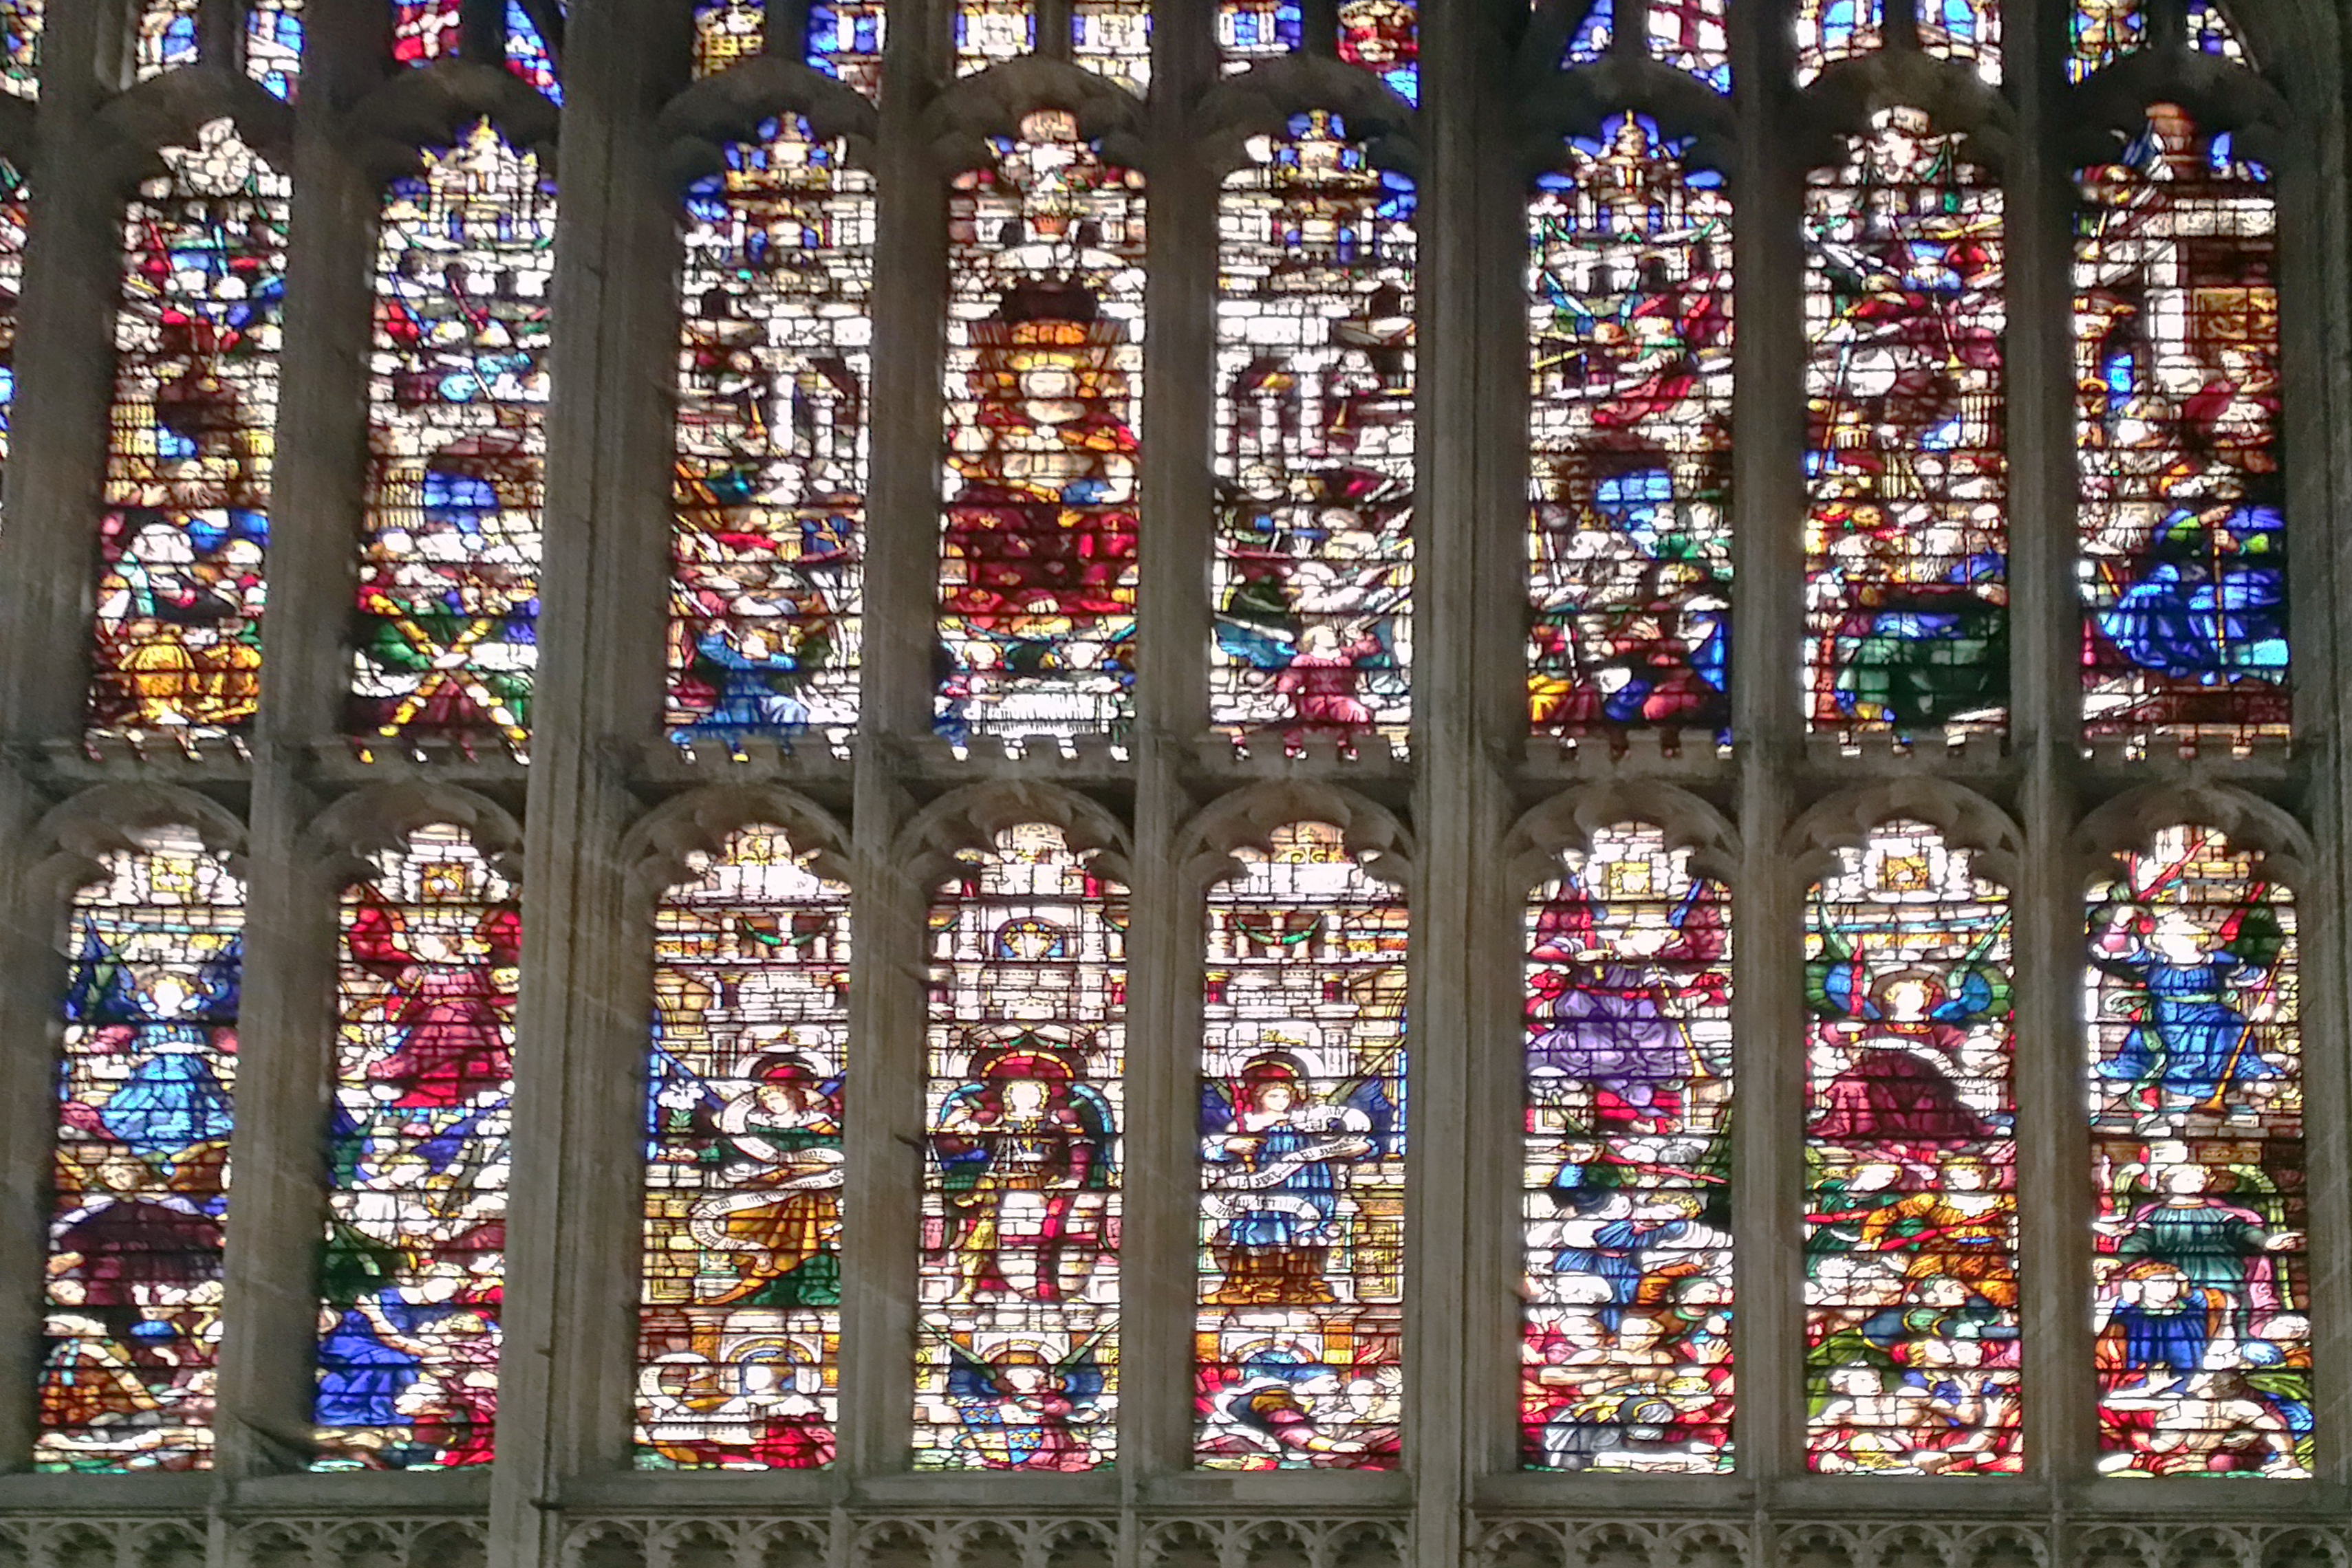
\includegraphics[width=0.5\textwidth,angle=0]{F2}
    \caption{From “Pacific Theater,” WWII, 1942-45 \\ 士兵受伤流血的手}
    \label{F-01}
\end{figure}

\section{Comments}
从第一幅照片中可以看出,米勒对于拍摄人的群体有自己的风格,在照片中,蒙巴顿上将并没有位于照片中央,也没有刻意被突出,
照片主要表现了海军人数众多,团结有力的压倒性的气势。

而从第二幅照片中,不难看出,米勒对于细节的把握也十分独到,照片中流血的手还握着钢盔,手臂上的止血带以及座椅上的药品,
虽然没有直接展示士兵的样貌,却可以展现军人坚强的意志,也反映美国军队后勤补给即医疗水平的强大。

笔者看来,韦恩$\cdot$米勒在他的照片中,既是尽可能的做到对二战期间美国军队的写实表达,
又通过艺术手法的应用,表达了自己对于祖国的自豪和对军人的敬佩等情感。

\bibstyle{unsrt}
\bibliography{references}{}
\end{document}
